% --------------------------------------------------------------------------- %
% Poster for the ECCS 2011 Conference about Elementary Dynamic Networks.      %
% --------------------------------------------------------------------------- %
% Created with Brian Amberg's LaTeX Poster Template. Please refer for the     %
% attached README.md file for the details how to compile with `pdflatex`.     %
% --------------------------------------------------------------------------- %
% $LastChangedDate:: 2011-09-11 10:57:12 +0200 (V, 11 szept. 2011)          $ %
% $LastChangedRevision:: 128                                                $ %
% $LastChangedBy:: rlegendi                                                 $ %
% $Id:: poster.tex 128 2011-09-11 08:57:12Z rlegendi                        $ %
% --------------------------------------------------------------------------- %
\documentclass[a0paper,portrait]{baposter}

\usepackage{relsize}		% For \smaller
\usepackage{url}			% For \url
\usepackage{epstopdf}	% Included EPS files automatically converted to PDF to include with pdflatex

%%% Global Settings %%%%%%%%%%%%%%%%%%%%%%%%%%%%%%%%%%%%%%%%%%%%%%%%%%%%%%%%%%%

\graphicspath{{pix/}}	% Root directory of the pictures 
\tracingstats=2			% Enabled LaTeX logging with conditionals

%%% Color Definitions %%%%%%%%%%%%%%%%%%%%%%%%%%%%%%%%%%%%%%%%%%%%%%%%%%%%%%%%%

\definecolor{bordercol}{RGB}{40,40,40}
\definecolor{headercol1}{RGB}{186,215,230}
\definecolor{headercol2}{RGB}{80,80,80}
\definecolor{headerfontcol}{RGB}{0,0,0}
\definecolor{boxcolor}{RGB}{186,215,230}

%%%%%%%%%%%%%%%%%%%%%%%%%%%%%%%%%%%%%%%%%%%%%%%%%%%%%%%%%%%%%%%%%%%%%%%%%%%%%%%%
%%% Utility functions %%%%%%%%%%%%%%%%%%%%%%%%%%%%%%%%%%%%%%%%%%%%%%%%%%%%%%%%%%

%%% Save space in lists. Use this after the opening of the list %%%%%%%%%%%%%%%%
\newcommand{\compresslist}{
	\setlength{\itemsep}{1pt}
	\setlength{\parskip}{0pt}
	\setlength{\parsep}{0pt}
}

%%%%%%%%%%%%%%%%%%%%%%%%%%%%%%%%%%%%%%%%%%%%%%%%%%%%%%%%%%%%%%%%%%%%%%%%%%%%%%%
%%% Document Start %%%%%%%%%%%%%%%%%%%%%%%%%%%%%%%%%%%%%%%%%%%%%%%%%%%%%%%%%%%%
%%%%%%%%%%%%%%%%%%%%%%%%%%%%%%%%%%%%%%%%%%%%%%%%%%%%%%%%%%%%%%%%%%%%%%%%%%%%%%%

\begin{document}
\typeout{Poster rendering started}

%%% Setting Background Image %%%%%%%%%%%%%%%%%%%%%%%%%%%%%%%%%%%%%%%%%%%%%%%%%%
\background{
	\begin{tikzpicture}[remember picture,overlay]%
	\draw (current page.north west)+(-2em,2em) node[anchor=north west]
	{
\includegraphics[height=1.1\textheight]{background}};
	\end{tikzpicture}
}

%%% General Poster Settings %%%%%%%%%%%%%%%%%%%%%%%%%%%%%%%%%%%%%%%%%%%%%%%%%%%
%%%%%% Eye Catcher, Title, Authors and University Images %%%%%%%%%%%%%%%%%%%%%%
\begin{poster}{
	grid=false,
	% Option is left on true though the eyecatcher is not used. The reason is
	% that we have a bit nicer looking title and author formatting in the headercol
	% this way
	%eyecatcher=false, 
	borderColor=bordercol,
	headerColorOne=headercol1,
	headerColorTwo=headercol2,
	headerFontColor=headerfontcol,
	% Only simple background color used, no shading, so boxColorTwo isn't necessary
	boxColorOne=boxcolor,
	headershape=roundedright,
	headerfont=\Large\sf\bf,
	textborder=rectangle,
	background=user,
	headerborder=open,
  boxshade=plain
}
%%% Eye Cacther %%%%%%%%%%%%%%%%%%%%%%%%%%%%%%%%%%%%%%%%%%%%%%%%%%%%%%%%%%%%%%%
{
	Eye Catcher, empty if option eyecatcher=false - unused
}
%%% Title %%%%%%%%%%%%%%%%%%%%%%%%%%%%%%%%%%%%%%%%%%%%%%%%%%%%%%%%%%%%%%%%%%%%%
{\sf\bf
	Properties of Elementary Random and Preferential Dynamic Networks
}
%%% Authors %%%%%%%%%%%%%%%%%%%%%%%%%%%%%%%%%%%%%%%%%%%%%%%%%%%%%%%%%%%%%%%%%%%
{
	\vspace{1em} Richard O. Legendi, Laszlo Gulyas, George Kampis\\
	{\smaller legendi@inf.elte.hu, lgulyas@colbud.hu, gkampis@colbud.hu}
}
%%% Logo %%%%%%%%%%%%%%%%%%%%%%%%%%%%%%%%%%%%%%%%%%%%%%%%%%%%%%%%%%%%%%%%%%%%%%
{
% The logos are compressed a bit into a simple box to make them smaller on the result
% (Wasn't able to find any bigger of them.)
\setlength\fboxsep{0pt}
\setlength\fboxrule{0.5pt}
	\fbox{
		\begin{minipage}{14em}
			
\includegraphics[width=10em,height=4em]{colbud_logo}
			
\includegraphics[width=4em,height=4em]{elte_logo} \\
			
\includegraphics[width=10em,height=4em]{dynanets_logo}
			
\includegraphics[width=4em,height=4em]{aitia_logo}
		\end{minipage}
	}
}

\headerbox{Problem}{name=problem,column=0,row=0}{
Sampling networks always involves the act of aggregation (e.g., when collecting longitudinal samples of networks). We sutdy how the cumulation window length effects the properties of the aggregated network.

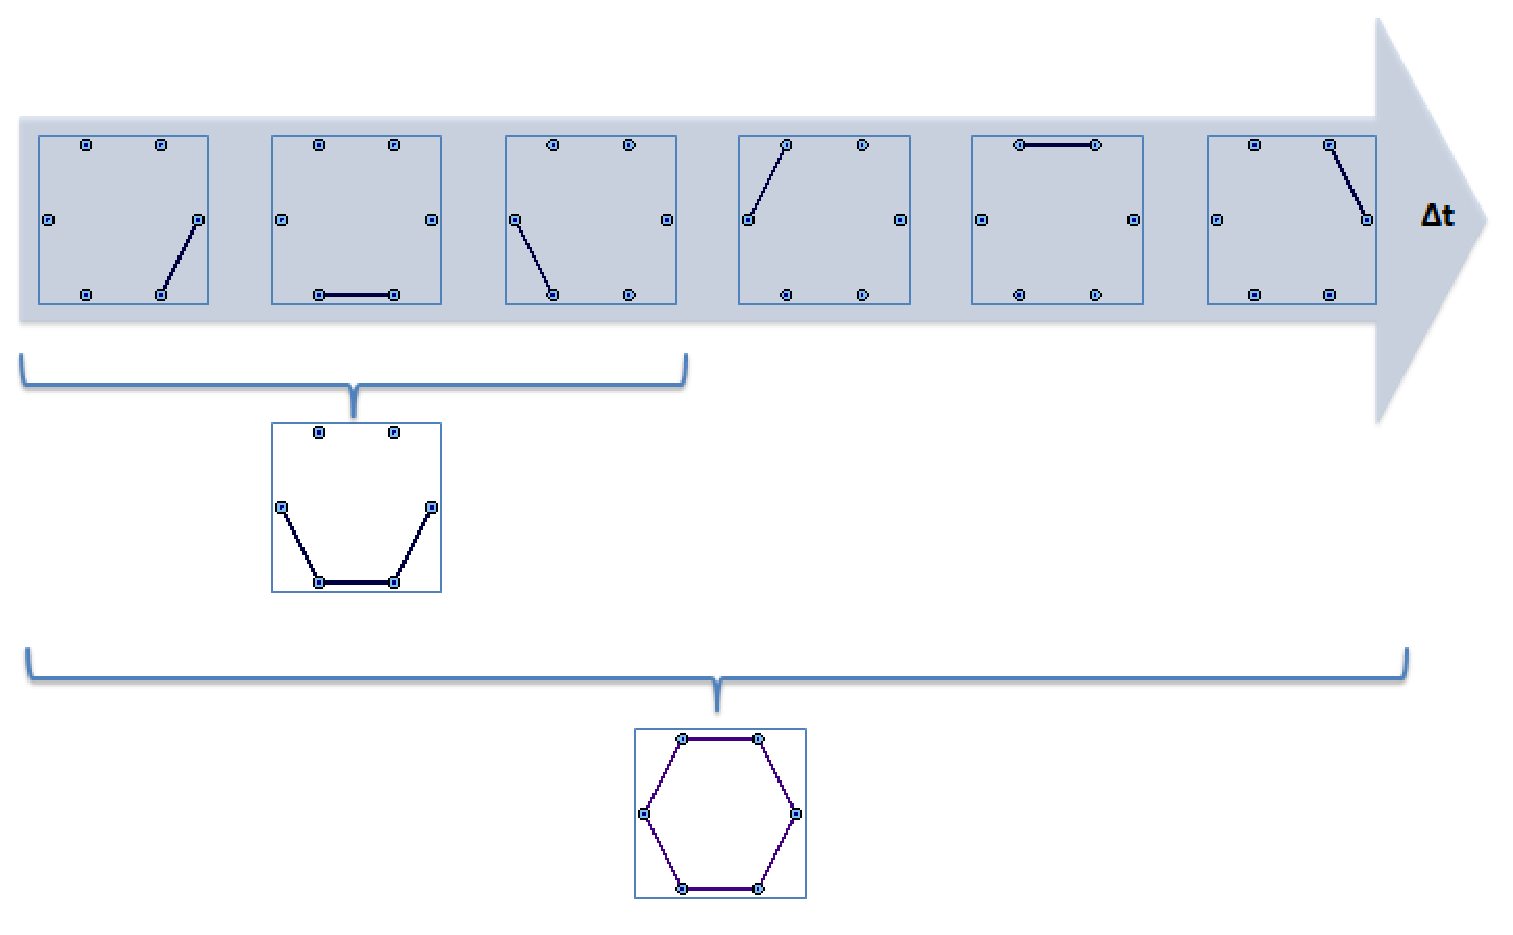
\includegraphics[width=\linewidth]{time_windows}
}

\headerbox{Basic Concepts}{name=definitions,column=0,below=problem}{
In our work the dynamic network is a series of graphs, that is, $DN = G_t(V_t,E_t)$, where $E_t \subseteq V_t \times V_t$ ($\forall t \geq 0$). The initial network, $G_0$, is considered as a parameter of the process. The \textbf{node set fixed} and we worked with an about \textbf{constant number of edges}. We assume that the evolution of the network can be described as the result of an edge creation and an edge deletion process. We define $G_t$ as the \textbf{snapshot network} and 
	{\smaller
	$$G_T = ( \bigcup^{T}_{t=0}V_t, \bigcup^{T}_{t=0}E_t) ~ \textnormal{for} ~ T \geq 0.$$
	}
as the \textbf{cumulative network}.
}

\headerbox{Models}{name=models,column=0,below=definitions}{
\textbf{ER1} $G_0$ is a random graph. Add each non-existing edge with $p_A$, delete each existing edge with $p_D$ probability. \\
\textbf{ER2} $G_0$ is a random graph. Add $k_A$ uniformly selected random new edges and delete $k_D$ existing edges. \\
\textbf{ER3} $G_0$ is a random graph. Rewire $k_{RW}$ edges. \\
\textbf{SPA} (\emph{Snapshot preferential}) $G_0$ is a scale free network. Add $k_A$ edges from a random node with preferential attachment based on the snapshot network. Delete $k_D$ existing edges. \\
\textbf{CPA} (\emph{Cumulative preferential}) $G_0$ is a scale free network. Add $k_A$ edges from a random node with preferential attachment based on the cumulative network. Delete $k_D$ existing edges.
}

\headerbox{References}{name=references,column=0,below=models}{
\smaller													% Make the whole text smaller
\vspace{-0.4em} 										% Save some space at the beginning
\bibliographystyle{plain}							% Use plain style
\renewcommand{\section}[2]{\vskip 0.05em}		% Omit "References" title
\begin{thebibliography}{1}							% Simple bibliography with widest label of 1
\itemsep=-0.01em										% Save space between the separation
\setlength{\baselineskip}{0.4em}					% Save space with longer lines
\bibitem{prevWork1} Laszlo Gulyas, Richard Legendi: \emph{Effects of Sample Duration on Network Statistics in Elementary Models of Dynamic Networks}, International Conference on Computational Science, Singapore (2011) 
\bibitem{prevWork2} Laszlo Gulyas, Susan Khor, Richard Legendi and George Kampis \emph{Cumulative Properties of Elementary Dynamic Networks}, The International Sunbelt Social Network Conference XXXI (2011)
\bibitem{gulya-kampis1} Gulyas, Laszlo et al.: \emph{Betweenness Centrality Dynamics in Networks of Changing Density}. Presented at the 19th International Symposium on Mathematical Theory of Networks and Systems (MTNS 2010)
\end{thebibliography}
}

\headerbox{Acknowledgements}{name=acknowledgements,column=0,below=references, above=bottom}{
\smaller						% Make the whole text smaller
\vspace{-0.4em}			% Save some space at the beginning
This research was partially supported by the Hungarian Government (KMOP-1.1.2-08/1-2008-0002 ) and the European Union's Seventh Framework Programme: DynaNets, FET-Open project no. FET-233847 (\url{http://www.dynanets.org}). The supports are gratefully acknowledged.
} 

\headerbox{Dynamic Networks are Sensitive to Aggregation}{name=density,span=2,column=1,row=0}{
Network characteristics are extremely sensitive to minor changes in aggregation length. In our previous work \cite{prevWork1} \cite{prevWork2}, we studied the cumulative properties of Elementary Dynamic Network models over the complete time period (i.e., until they reach the stable point of a full network). Here we focus on the more realistc domain of sparse (cumulative) networks. We find that even when snapshot networks are stationary, \textbf{important network characteristics}  (average path lenght, clustering, betwenness centrality) \textbf{are extremely sensitive to aggregation} (window length). 

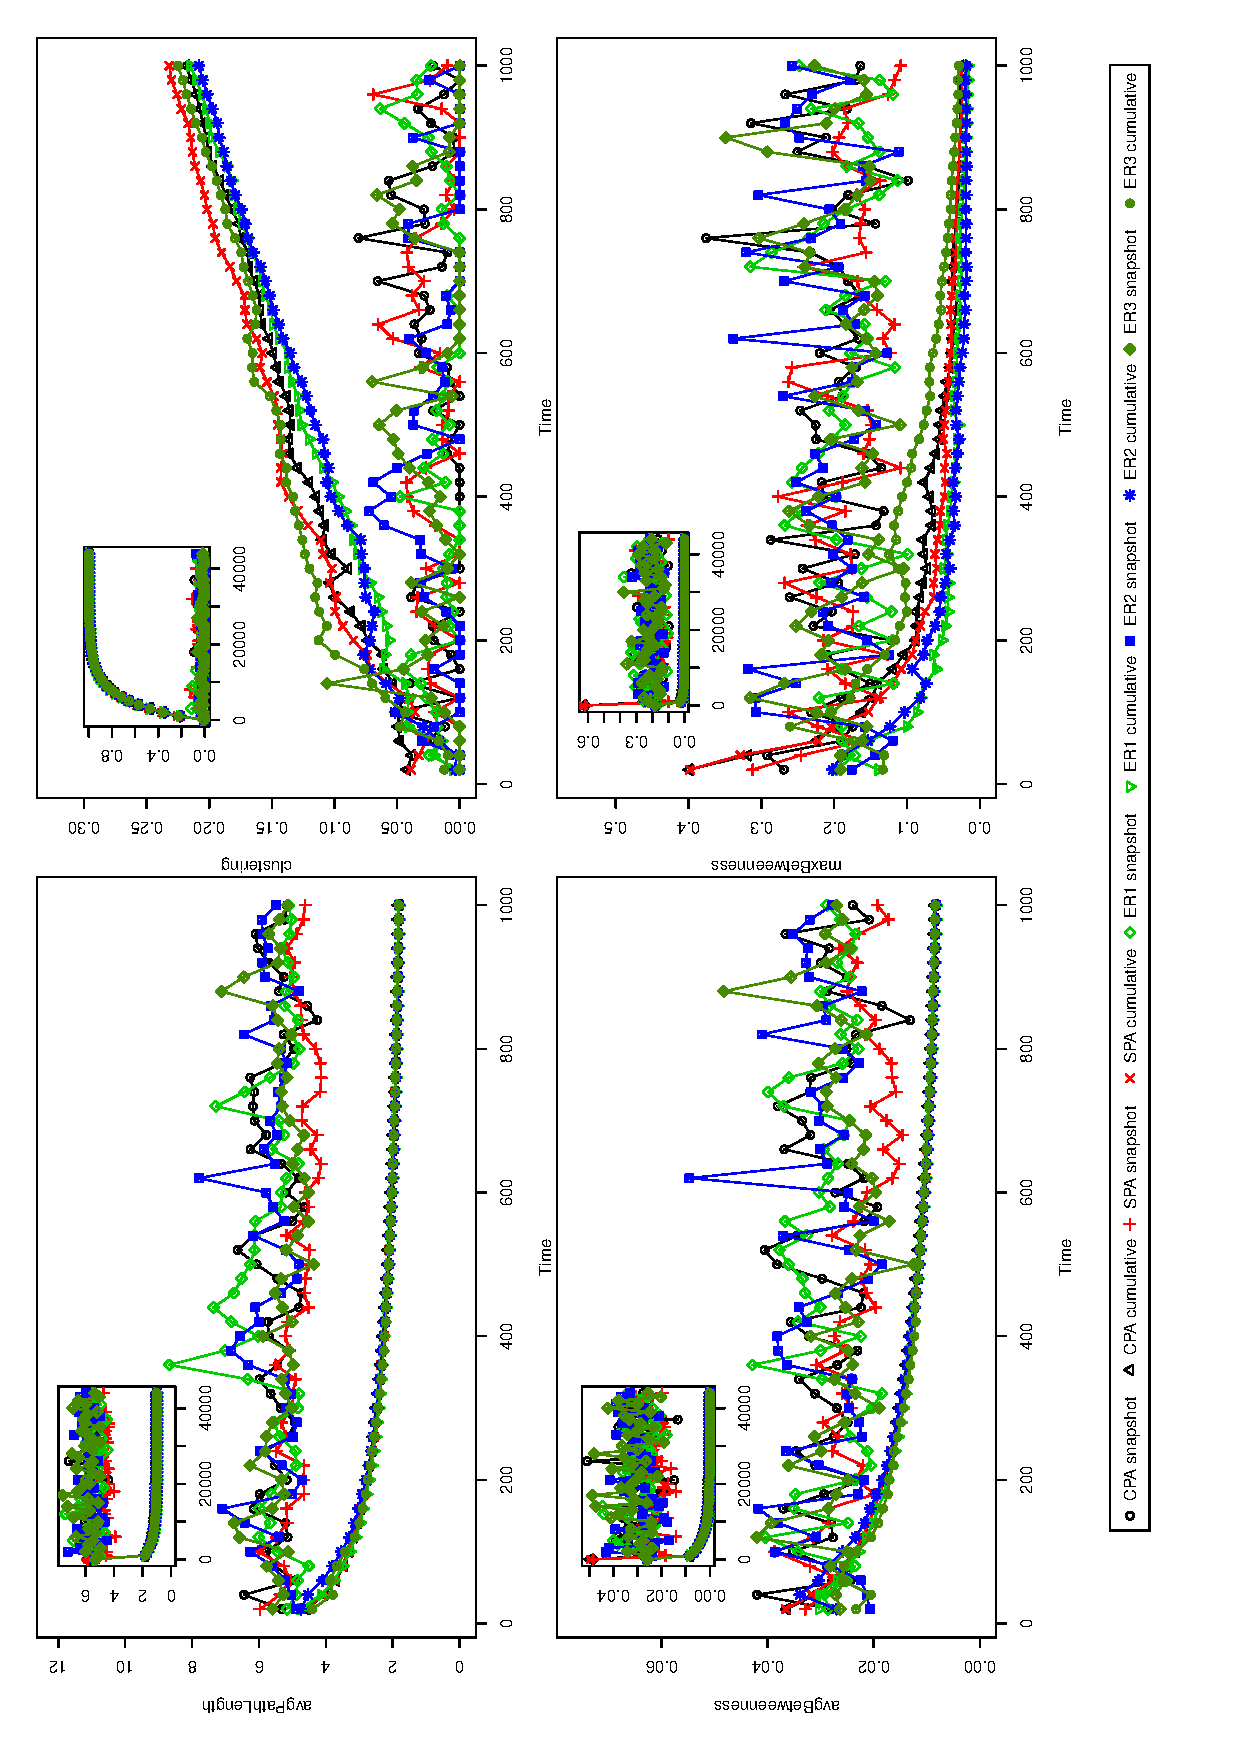
\includegraphics[angle=-90,width=0.98\linewidth]{PA_and_ER_Models_statisticalMeasures}
}

\headerbox{Degree Distribution Radically Changes}
{name=degreeDistribution,span=2,column=1,below=density,above=bottom}{
Degree distributions are exceptionally sensitive to the length of the aggregation window. \textbf{The same dynamic network may produce a normal, lognormal or even power law distribution for different aggregation lenghts.} The digree distribution of the snapshot and cumulative network is inherently different. The following surfaces show the CPA model until it approaches the complete network.
\vspace{-0.2em}
\begin{center}
	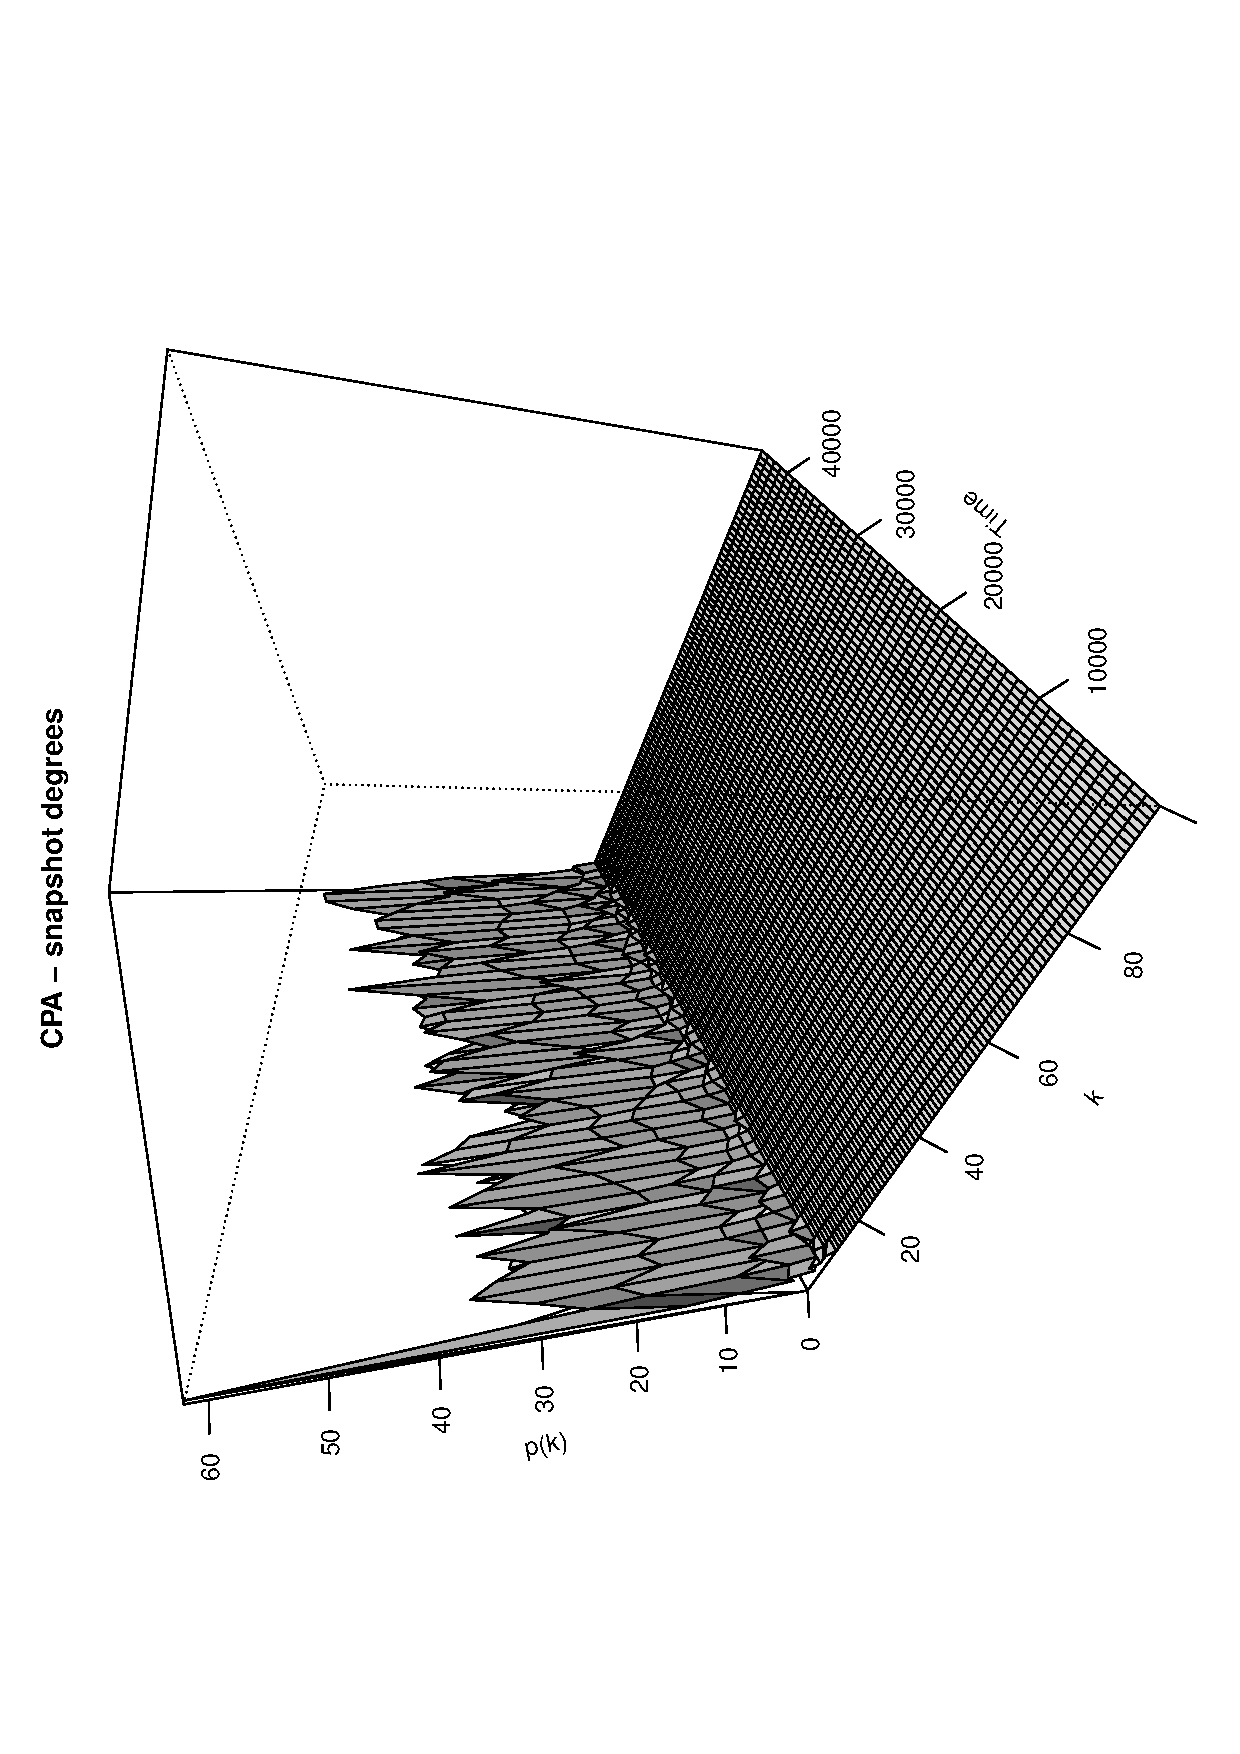
\includegraphics[angle=-90,width=0.49\linewidth]{CPA_3d_snapshot}
	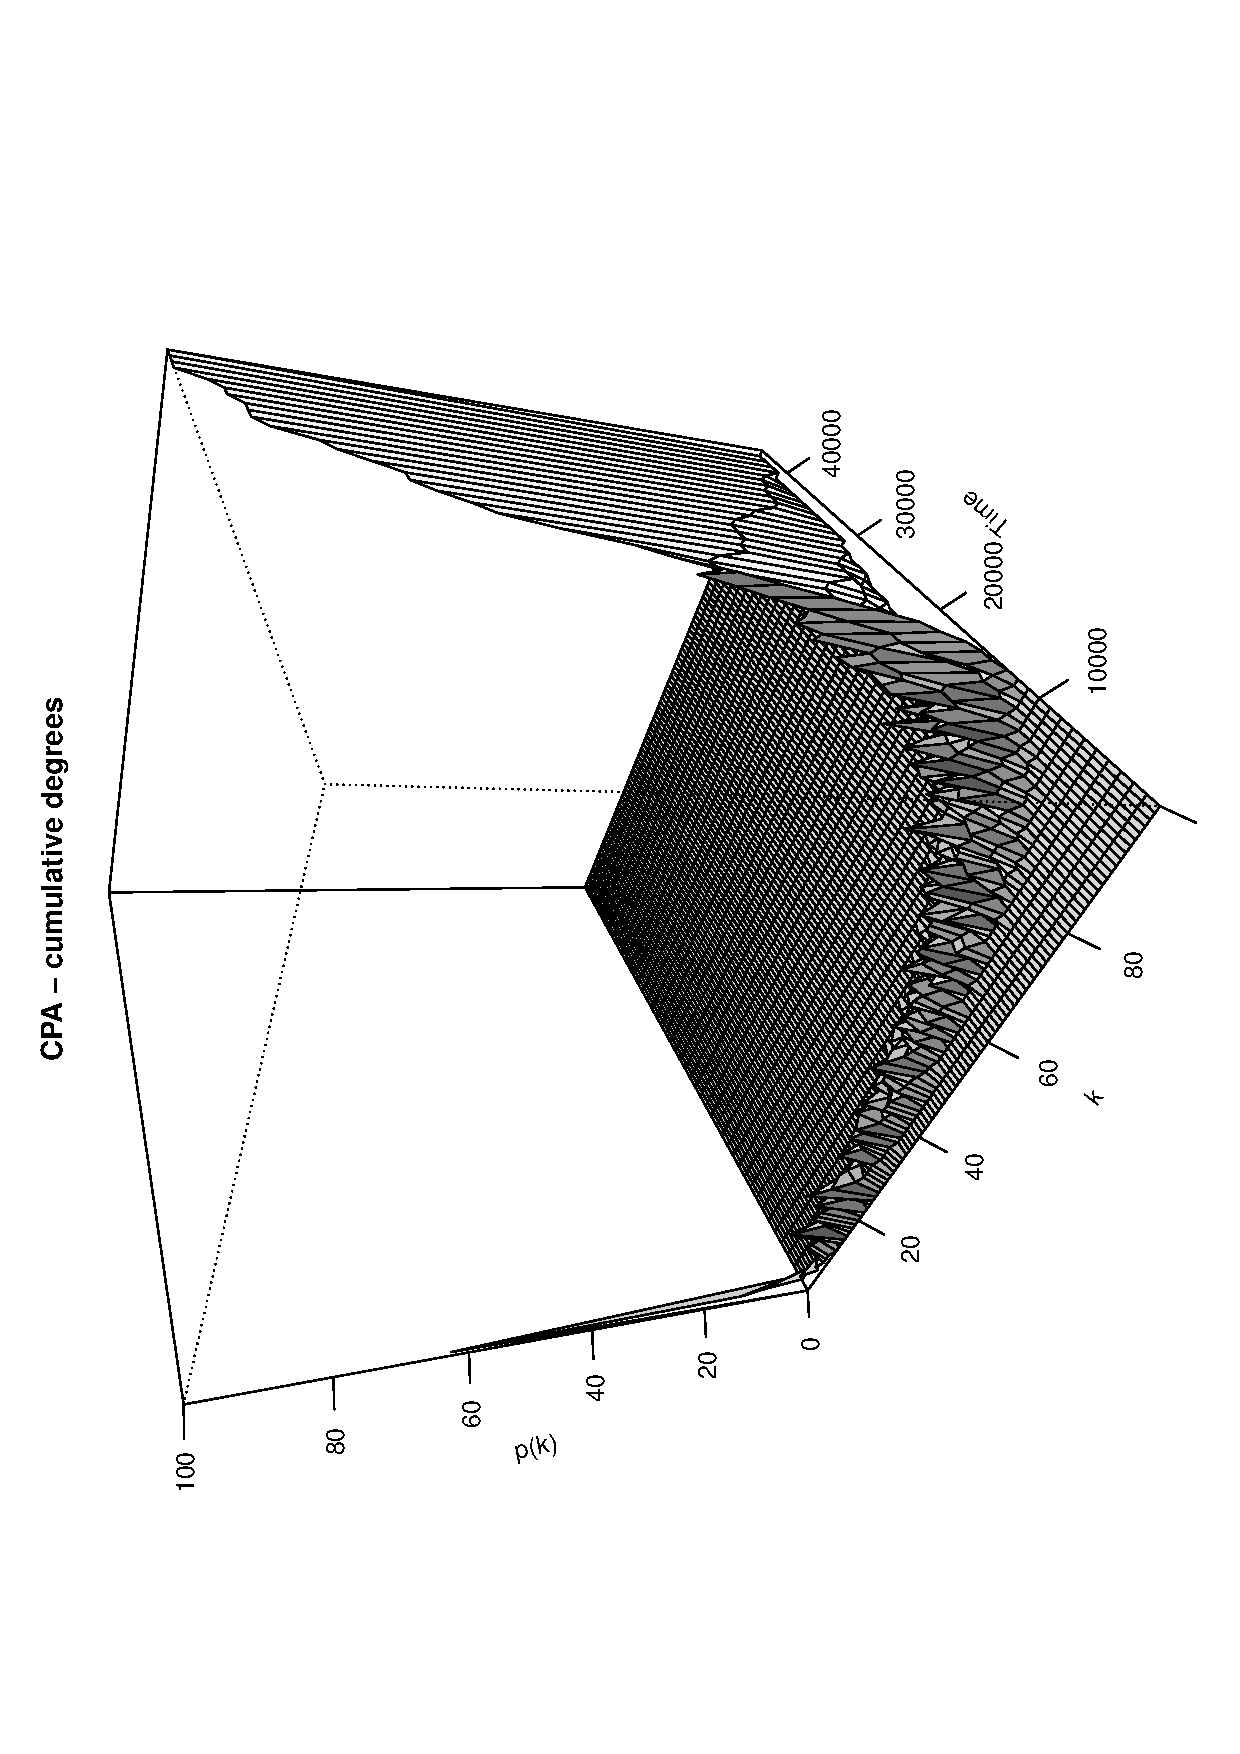
\includegraphics[angle=-90,width=0.49\linewidth]{CPA_3d_cumulative}
\end{center}
\vspace{-0.2em}
Taking slices of the cumulative 3D charts shows us how the degree distribution changes. The log-log charts below show the progression of these changes as the aggregation window gets larger.
\vspace{-0.2em}
\begin{center}
	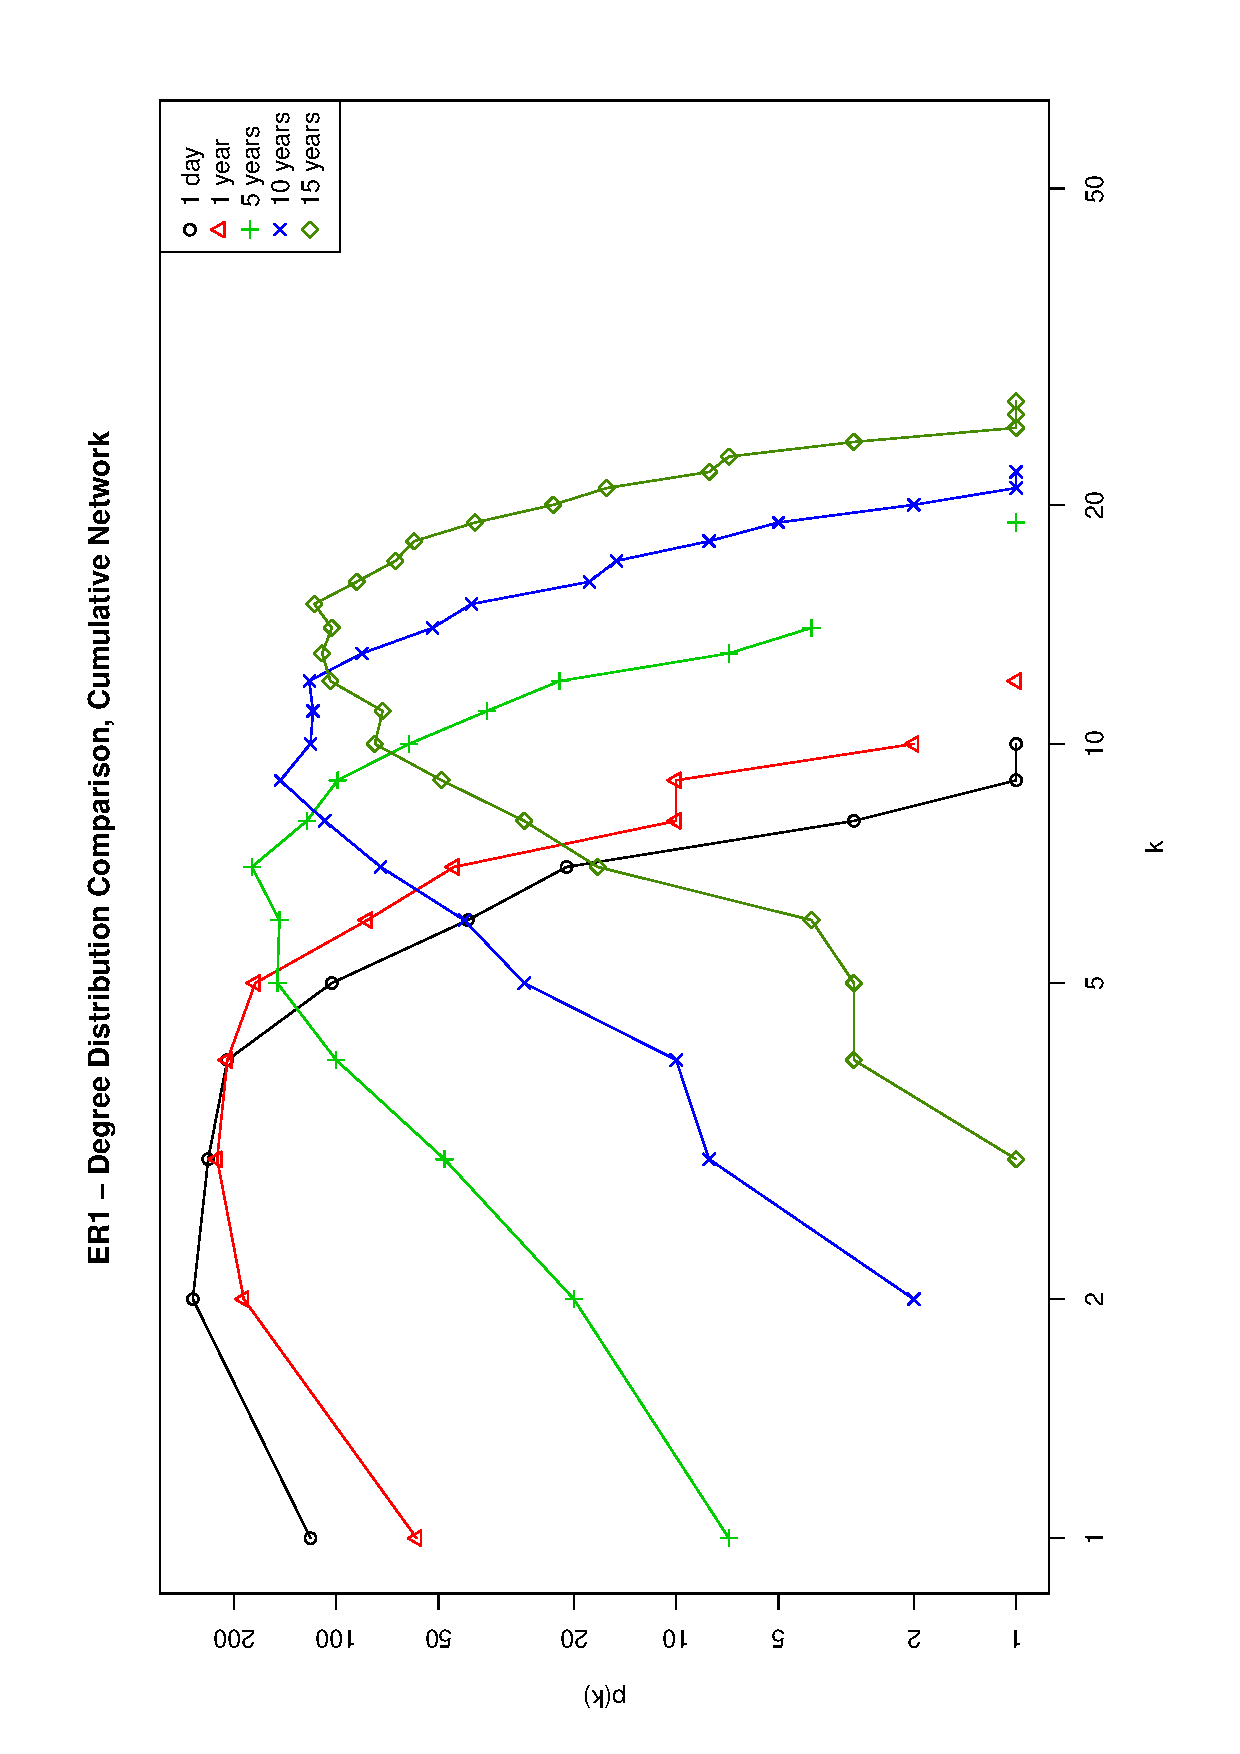
\includegraphics[angle=-90,width=0.49\linewidth]{ER1_cumulativeDegrees}
	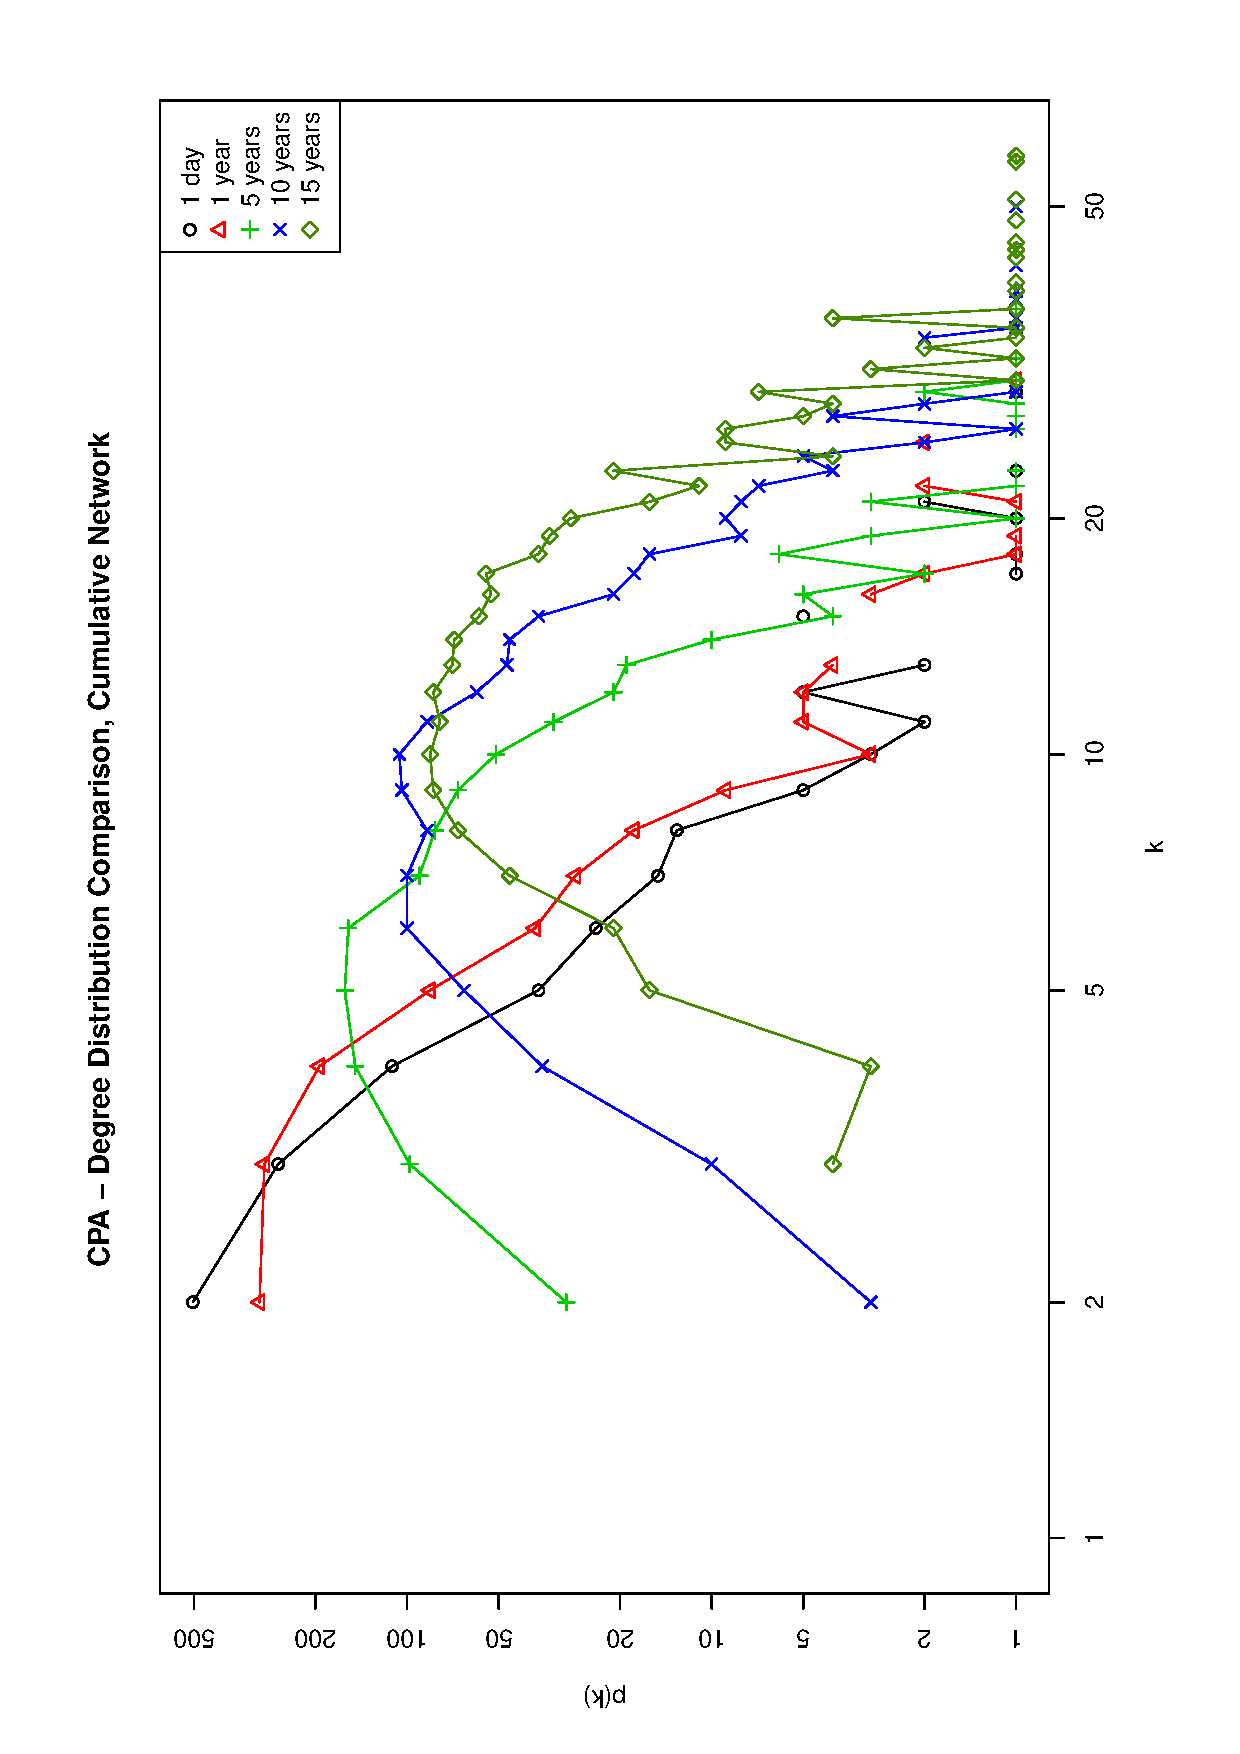
\includegraphics[angle=-90,width=0.49\linewidth]{CPA_cumulativeDegrees}
\end{center}
}

\end{poster}
\end{document}
